\clearpage \section{Application}

This last section of the chapter aims to present the entire application that was developed in the course of this thesis. The source code for the application, as well as the Jupyter Notebook in which the data mining part was implemented, can be found as a \emph{Git} repository on \emph{GitHub} under the following link:

\begin{quote}
    \centering
    \underline{https://github.com/jakobheine/fm-analytics/tree/v.1.0.0}
\end{quote}

As already mentioned at the beginning of this chapter, the application is implemented in a microservice architecture. All services are created as \emph{Docker} containers, which makes them easy to deploy. The entire tool is deployed on a virtual private server (VPS) hosted on Hetzner.\parencite[][]{hetzner_about_2021} The following figure shows the architecture and how the microservices interact with each other.

\begin{figure}[H]
    \centering
    \fbox{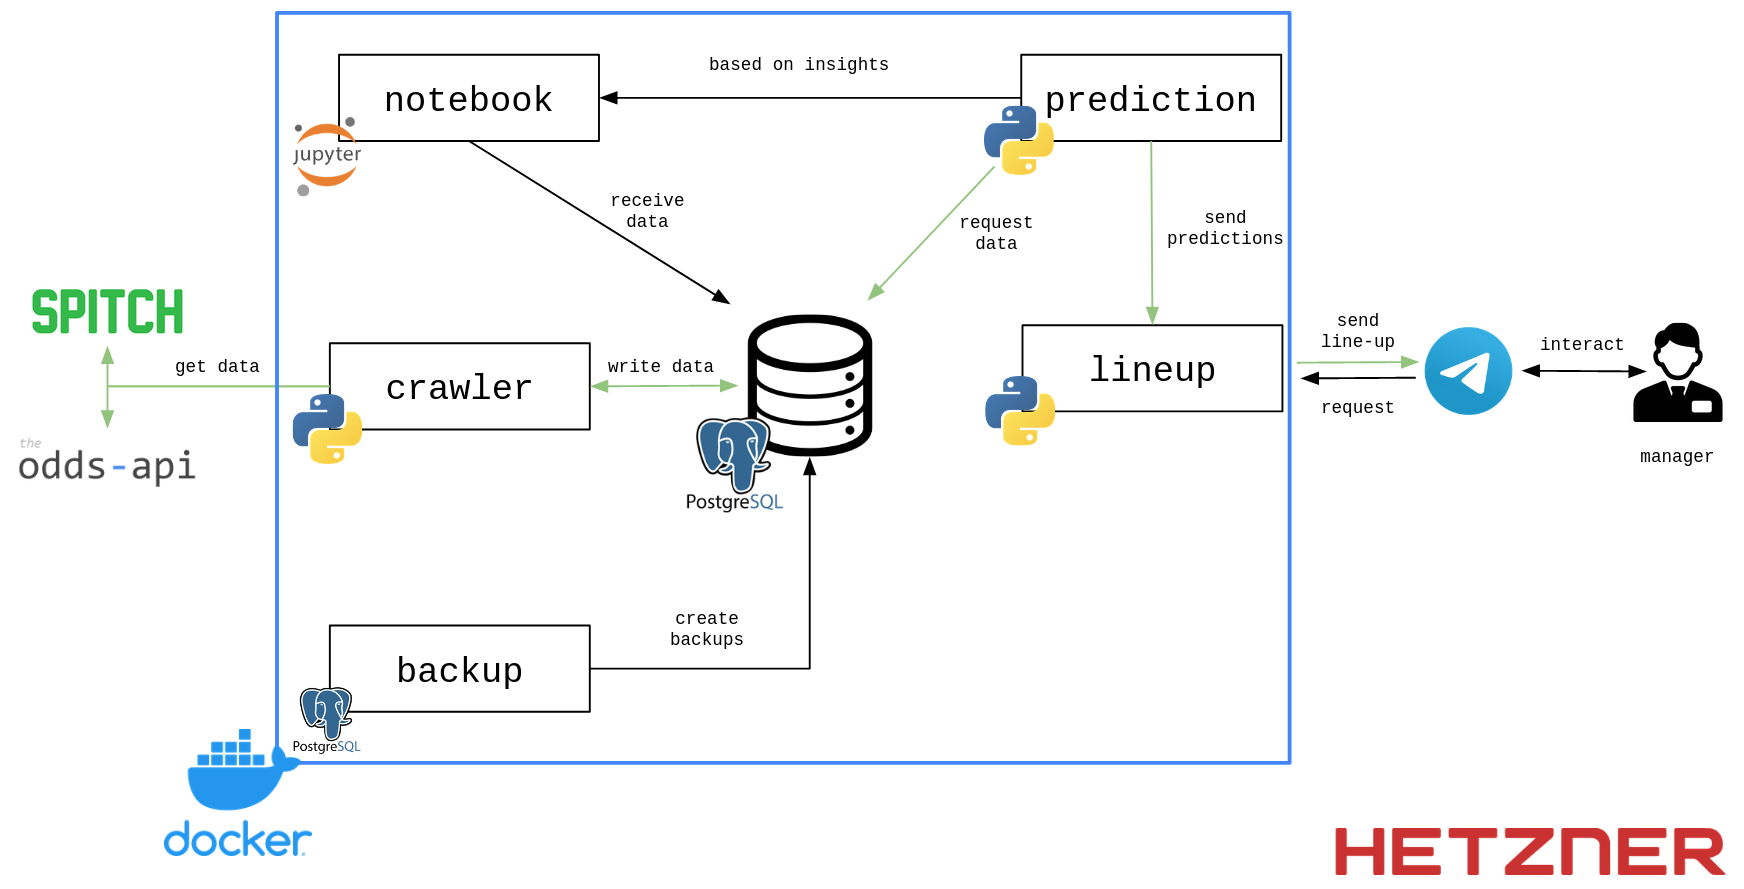
\includegraphics[width=15cm]{chapter/4_implementation/figures/microservice-architecture.png}}
    \captionsetup{justification=centering}
    \caption{Microservice-Architecture of the Application}
    \label{fig:microservice-architecture}
\end{figure}

The green arrows indicate the primary process. In this process, the \emph{Crawler} collects the current data from \emph{SPITCH} and \emph{the odds-api} via the \emph{Proxy} and stores it in the \emph{Database}. This data is then queried by the \emph{Prediction} service, which predicts the individual scores of the players based on the findings from the \emph{Jupyter Notebook} and forwards them to the \emph{Lineup} service. The \emph{Lineup} service creates the optimal line-up from the predicted scores and the transfer market values, which it then sends to the end-users via a \emph{Telegram Bot}. This process starts 15 minutes before the kick-off of a matchday so that the data is as up-to-date as possible, but the managers still have enough time to line up the team predicted by the tool. In addition, the manager can start the process himself at any time. Furthermore, the \emph{Backup} service creates a backup of the database every 24 hours.

To deploy the application, only a server with \emph{Docker}, \emph{Docker-Compose}, and \emph{Git} installed is needed. After the \emph{Github} repository has been cloned, the application can be started with the command:  \lstinline{docker-compose up}.

The following screenshot shows the messages the application is sending to its users.

\begin{figure}[H]
    \centering
    \fbox{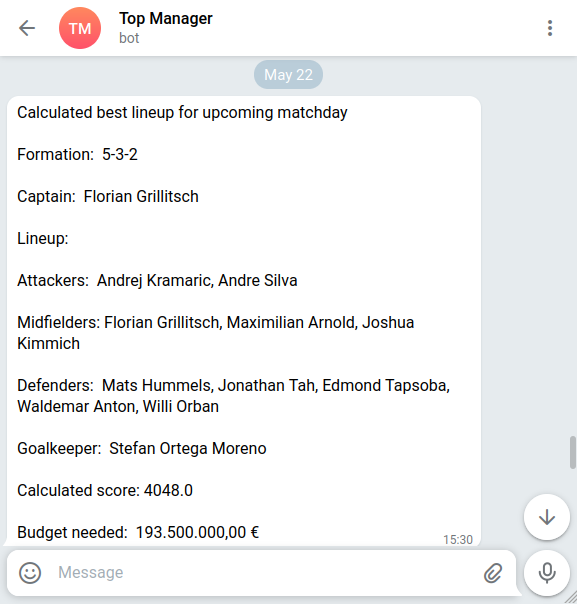
\includegraphics[width=12cm]{chapter/4_implementation/figures/telegram-message.png}}
    \captionsetup{justification=centering}
    \caption{Screenshot of the Applications Messages}
    \label{fig:screenshot-telegram}
\end{figure}